\section{Optimal solution to a path}
\subsection{Modeling of the physical system}
\begin{frame}{Physical system}
Modeling the physical system, of an EV and a path.
\begin{figure}[!htb]
\centering
    \begin{tikzpicture}[shorten >=1pt,node distance=2.5cm,>=stealth',thick]
        \node[state] (1) {$u_1$};
        \node[state] (2) [right of=1] {$u_2$};
        \node[] (dots) [right of=2] {$\dots$};
        \node[state] (n) [right of=dots] {$u_n$};
        \node[state,draw=none] (d1) [right of=n] {};
        \draw [->] (1) to[right] node[auto] {$e_1$} (2);
        \draw [->] (2) to[right] node[auto] {$e_2$} (dots);
        \draw [->] (dots) to[right] node[auto] {$e_{n-1}$} (n);
        %\draw [->] (n) to[right] node[auto] {$e_n$} (d1);
    \end{tikzpicture}
\end{figure} 
\begin{itemize}
\item Path
\begin{itemize}
\item[+] Charging stations, with charging rate ($R_{CH}(u_i)$)
\item[+] Road segments, with speed limit ($v_{min}(e_i)$, $v_{max}(e_i)$) and distance ($D(e_i)$) 
\end{itemize}
\item EV
\begin{itemize}
\item[+] Driving consumes energy accordingly to the speed of the EV, defined by: ($R_{CO}(e_i)$)
\item[+] Further two constants from the EV are important to model, namely, battery capacity ($B_{max}$) and initial battery ($B_{cur}$)
\end{itemize}
\end{itemize} 
\end{frame}
\subsection{Optimisation problem}
\begin{frame}{Optimisation problem}
Formulating a optimisation problem, which when solved will yield a optimal solution. 
\begin{itemize}
\item Objective: Move from $u_1$ to $u_n$ using minimum time . 
\begin{itemize}
\item[+] Time can be used driving or charging. 
\begin{itemize}
\item[-] $\text{min: } \sum_{i=1}^{n-1} \left(\frac{D(e_i)}{v_{e_i}} + CT_{u_i} \right)$
\end{itemize}
\end{itemize}
\item Physical constraints:
\begin{itemize}
\item[+] Each edge must be driven at a speed within the speed limit:\begin{itemize}
\item [-] $\forall_{i\in1 \dots n-1 }:\;v_{min}(e_i) \leq v_{e_i} \leq v_{max}(e_i)$
\end{itemize}
\item[+] Time can only be positive.\begin{itemize}
\item [-] $\forall_{i\in1 \dots n }:\; 0 \leq CT_{u_i} $
\end{itemize}

\item[+] The energy is the battery must alway be between 0 and $B_{max}$
\end{itemize}
\end{itemize} 
\end{frame}
\begin{frame}{battery constraint}
The battery constraint of the optimisation problem can be split into two parts
\begin{itemize}
\item No road segment can be passed without having the required energy
\item No overcharging at any charging station. 
\end{itemize}
Energy can be..
\begin{itemize}
\item Spend: $\forall_{i\in1 \dots n-1 }:\; ES(e_i) = D(e_i) \times R_{CO}(v_{e_i})$
\item Acuried: $\forall_{i\in1 \dots n }:\; EA(u_i) = R_{CH}(u_i) \times CT_{u_i}$
\item Already in the battery: $B_{cur}$
\end{itemize}
\end{frame}
\begin{frame}{battery constraint}
No road segment can be passed without having the required energy 
\begin{figure}[!htb]
\centering
    \begin{tikzpicture}[shorten >=1pt,node distance=2.5cm,>=stealth',thick]
        \node[state] (1) {$u_1$};
        \node[state] (2) [right of=1] {$u_2$};
        \node[] (dots) [right of=2] {$\dots$};
        \node[state] (n) [right of=dots] {$u_n$};
        \node[state,draw=none] (d1) [right of=n] {};
        \draw [->] (1) to[right] node[auto] {$e_1$} (2);
        \draw [->] (2) to[right] node[auto] {$e_2$} (dots);
        \draw [->] (dots) to[right] node[auto] {$e_{n-1}$} (n);
        %\draw [->] (n) to[right] node[auto] {$e_n$} (d1);
        \draw[decorate,decoration={brace,amplitude=5pt,mirror}] 
    (-0.5,-0.5) coordinate (1) -- (2,-0.5) coordinate (2);
    \node at (0.8,-1.0){$i=1$};
     \draw[decorate,decoration={brace,amplitude=5pt,mirror}] 
    (-0.5,-1.5) coordinate (1) -- (4.5,-1.5) coordinate (2);
    \node at (2.1,-2.0){$i=2$};
    \draw [dashed] (2.5,-2.5) -- (4,-2.5);
     \draw[decorate,decoration={brace,amplitude=5pt,mirror}] 
    (-0.5,-3.5) coordinate (1) -- (7,-3.5) coordinate (2);
    \node at (3.4,-4.0){$i=n-1$};

    \end{tikzpicture}
\end{figure} 
\begin{itemize}
\item $\forall_{i\in1 \dots n-1 }:\;0 \leq B_{cur} + \sum_{j=1}^{i} EA(u_j) - \sum_{j=1}^{i} ES(e_j) \leq B_{max}$
\end{itemize}
\end{frame}

\begin{frame}{battery constraint}
No overcharging at any charging station.
\begin{figure}[!htb]
\centering
    \begin{tikzpicture}[shorten >=1pt,node distance=2.5cm,>=stealth',thick]
        \node[state] (1) {$u_1$};
        \node[state] (2) [right of=1] {$u_2$};
        \node[] (dots) [right of=2] {$\dots$};
        \node[state] (n) [right of=dots] {$u_n$};
        \node[state,draw=none] (d1) [right of=n] {};
        \draw [->] (1) to[right] node[auto] {$e_1$} (2);
        \draw [->] (2) to[right] node[auto] {$e_2$} (dots);
        \draw [->] (dots) to[right] node[auto] {$e_{n-1}$} (n);
        %\draw [->] (n) to[right] node[auto] {$e_n$} (d1);
        \draw[decorate,decoration={brace,amplitude=5pt,mirror}] 
    (-0.5,-0.5) coordinate (1) -- (3,-0.5) coordinate (2);
    \node at (1.3,-1.0){$i=1$};
     \draw[decorate,decoration={brace,amplitude=5pt,mirror}] 
    (-0.5,-1.5) coordinate (1) -- (5.5,-1.5) coordinate (2);
    \node at (2.6,-2.0){$i=2$};
    \draw [dashed] (3,-2.5) -- (6.5,-2.5);
     \draw[decorate,decoration={brace,amplitude=5pt,mirror}] 
    (-0.5,-3.5) coordinate (1) -- (8,-3.5) coordinate (2);
    \node at (3.9,-4.0){$i=n-1$};

    \end{tikzpicture}
\end{figure} 
\begin{itemize}
\item $\forall_{i\in1 \dots n-1}:\;0 \leq B_{cur} + \sum_{j=1}^{i+1} EA(u_j) - \sum_{j=1}^{i} ES(e_j) \leq B_{max}$
\end{itemize}
\end{frame}
\subsection{Linear programming}
\begin{frame}{Linear programming}
NP-complete problem.

Linearization and linear programming for approximate solution. 

Two functions of the optimisation problem are non linear functions. 
\begin{itemize}
\item Consumption rate ($R_{CO}(v_{e_i})$)
\item Driving time ($\frac{D(e_i)}{v_{e_i}}$)
\end{itemize}
\end{frame}


\begin{frame}{linearization example}
Function for energy consumption before linearization. $R_{CO}(v)=0.019*x^2 - 0.770*x + 184.4$
\begin{figure}[!htb]
\label{fig:graph}
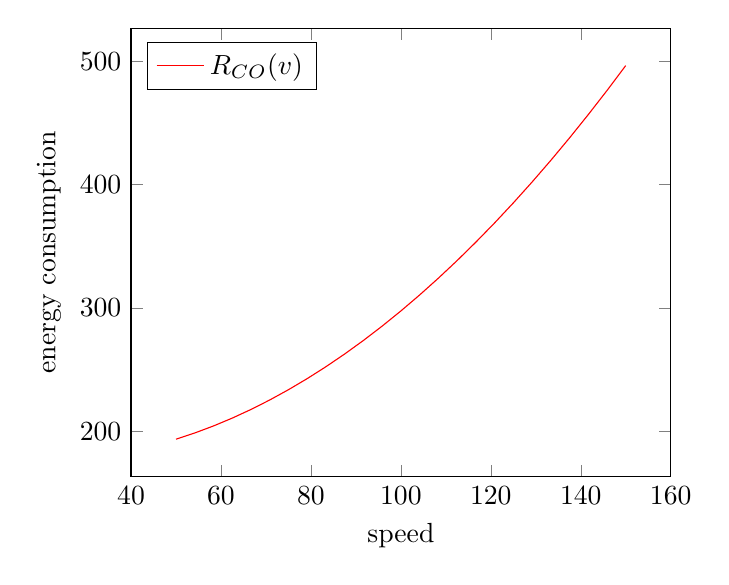
\begin{tikzpicture}
\begin{axis}[xlabel=speed, ylabel=energy consumption,legend style={legend pos=north west}]
\addplot[draw=red,domain=50:150]{(0.019*x^2 - 0.770*x + 184.49) };
\addlegendentry{$R_{CO}(v)$}

% \addplot[mark=*, domain=25:75] coordinates {(37,295)};
\end{axis}
\end{tikzpicture}% 

\label{fig:graph}
\end{figure}
\end{frame}

\begin{frame}{linearization example}
Function for energy consumption after linearization. $R_{CO}(v)=0.019*x^2 - 0.770*x + 184.4$
\begin{figure}[!htb]
\label{fig:graph}
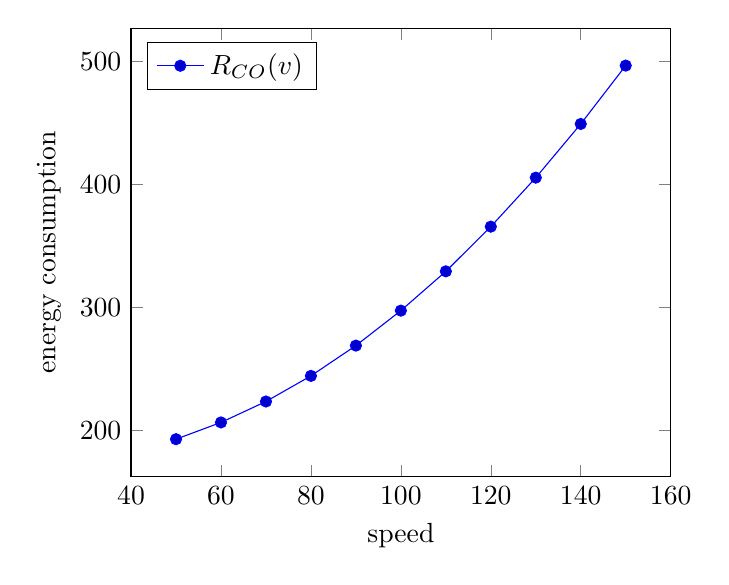
\begin{tikzpicture}
\begin{axis}[xlabel=speed, ylabel=energy consumption,legend style={legend pos=north west}]
\addplot coordinates { (50,193) (60,206.6) (70,223.6) (80,244.4) (90,269) (100,297.4) (110,329.3) (120,365.6) (130,405.4) (140, 449) (150,496.4) }; \addlegendentry{$R_{CO}(v)$ }

% \addplot[mark=*, domain=25:75] coordinates {(37,295)};
\end{axis}
\end{tikzpicture}% 

\label{fig:graph}
\end{figure}
\begin{itemize}
\item For all linear function their slope and the y-intercept is precomputed. 
\item For every edge in the path exactly one line segment needs to be chosen. Thus a binary matrix i introduced of size $n \times m$, where $n$ is edges in the path and $m$ is linear pieces of each line. 
\end{itemize}
\end{frame}
\begin{frame}{linearization example}
\begin{itemize}
\item For all linear function their slope and the y-intercept is precomputed. 
\item For every edge in the path exactly one line segment needs to be chosen. Thus a binary matrix i introduced of size $n \times m$, where $n=$edges in the path and $m=$linear pieces of each line. 
\end{itemize}
\end{frame}



